% =====================================================================
%  Resolução de exercícios — Sistemas Elétricos de Potência
%  Questões 51 (abertura de linha), 24 (fluxo de potência) e 45 (potência
%  ativa e reativa a partir da potência instantânea)
%  Compilar com pdflatex (funciona no Overleaf sem ajustes)
% =====================================================================
\documentclass[aspectratio=169,11pt]{beamer}

\usepackage[utf8]{inputenc}
\usepackage[T1]{fontenc}
\IfFileExists{portuges.ldf}{\usepackage[brazil]{babel}}{}
\usepackage{amsmath,amssymb}
\usepackage{icomma}            % vírgula decimal em modo matemático: 0,5
\usepackage{booktabs}
\usepackage[american,cuteinductors]{circuitikz}
\usepackage{tcolorbox}
\usetikzlibrary{arrows.meta,calc}
\usepackage{pgfplots}          % gráfico da potência instantânea (Q45)
\pgfplotsset{compat=1.18}
\providecommand{\sen}{\operatorname{sen}}   % "sen", como no enunciado da Q45
% bibliografia: mesmas opções do template GREI (biber; latexmk roda sozinho)
\usepackage{csquotes}
\usepackage[backend=biber,style=numeric,sorting=none]{biblatex}
\addbibresource{referencias.bib}
% deixa a URL quebrar em qualquer letra/número (sem isso ela vaza da margem)
\setcounter{biburllcpenalty}{7000}
\setcounter{biburlucpenalty}{8000}
\setcounter{biburlnumpenalty}{9000}

% ---------------------------------------------------------------------
%  Tema e cores
% ---------------------------------------------------------------------
\usetheme[progressbar=frametitle,numbering=fraction]{metropolis}
% allowframebreaks: numeral (ii, iii...) só a partir do 2º slide; precisa vir
% depois do \usetheme, que define o seu próprio
\setbeamertemplate{frametitle continuation}[from second][\romannumeral\insertcontinuationcount]
\definecolor{Navy}{HTML}{1D3557}
\definecolor{Teal}{HTML}{2A7F8E}
\definecolor{Ember}{HTML}{D1495B}
\definecolor{Paper}{HTML}{FAFAF7}
\definecolor{Ink}{HTML}{22262B}
\definecolor{Mute}{HTML}{7A828C}
% zonas de tensão base (Q51): cores alternadas entre zonas vizinhas
\colorlet{ZonaA}{Teal}
\colorlet{ZonaB}{Navy}
% Q45: potência ativa (média) e aparente (amplitude) no gráfico
\colorlet{CorP}{Teal}
\colorlet{CorS}{Ember}

\setbeamercolor{normal text}{fg=Ink,bg=Paper}
\setbeamercolor{frametitle}{fg=Paper,bg=Navy}
\setbeamercolor{progress bar}{fg=Ember,bg=Navy!40}
\setbeamercolor{alerted text}{fg=Ember}
\setbeamercolor{title separator}{fg=Ember}
\setbeamercolor{block title}{fg=Paper,bg=Teal}
\setbeamercolor{block body}{bg=Teal!8}
\setbeamertemplate{itemize item}{\color{Teal}$\blacktriangleright$}

% caixa de resposta
\newtcolorbox{resposta}[1][]{colback=Ember!7,colframe=Ember,boxrule=0.8pt,
  arc=2pt,left=6pt,right=6pt,top=4pt,bottom=4pt,#1}
% rótulo de passo
\newcommand{\passo}[1]{{\color{Teal}\bfseries #1}\enspace}

% ---------------------------------------------------------------------
%  Símbolos para diagramas unifilares (TikZ puro)
% ---------------------------------------------------------------------
\tikzset{
  barra/.style={line width=2.2pt,Ink},
  fio/.style={line width=0.8pt,Ink},
  gerador/.pic={
    \draw[fio,fill=white] (0,0) circle (0.36);
    \draw[fio] (-0.2,0) sin (-0.1,0.12) cos (0,0) sin (0.1,-0.12) cos (0.2,0);
  },
  trafo/.pic={
    \draw[fio] (-0.62,0) -- (-0.44,0) (0.44,0) -- (0.62,0);
    % enrolamentos iguais: fundo branco nos dois (como o gerador) e os dois
    % contornos por cima, para nenhum círculo encobrir o outro
    \fill[white] (-0.17,0) circle (0.27) (0.17,0) circle (0.27);
    \draw[fio] (-0.17,0) circle (0.27) (0.17,0) circle (0.27);
  },
  rot/.style={font=\footnotesize,Ink},
  rotb/.style={font=\scriptsize,Mute},
  numbarra/.style={circle,draw=Ink,line width=0.6pt,inner sep=1.2pt,
                   font=\scriptsize,fill=white},
}
\ctikzset{bipoles/length=1.05cm}

% ---------------------------------------------------------------------
%  Desenho do unifilar da Questão 51 (enunciado e zonas)
%  #1 = escala do tikzpicture onde é usado. O raio dos círculos dos pics
%  (gerador/trafo) não acompanha o scale, então os rótulos G e T ficam a
%  raio/escala abaixo do centro para não encostar neles.
% ---------------------------------------------------------------------
\newcommand{\circuitoQcinquentaum}[1]{%
  \pgfmathsetmacro{\dG}{0.36/#1}%
  \pgfmathsetmacro{\dT}{0.30/#1}%
  % geradores
  \draw[fio] (0.36,2) -- (1.2,2);   \pic at (0,2) {gerador};
  \node[rot,anchor=north] at (0,2-\dG) {$G_1$};
  \draw[fio] (9.6,2) -- (10.44,2);  \pic at (10.8,2) {gerador};
  \node[rot,anchor=north] at (10.8,2-\dG) {$G_2$};
  % barras
  \foreach \x in {1.2,3.6,7.2,9.6} \draw[barra] (\x,0.55) -- (\x,3.45);
  \node[rot,above] at (1.2,3.45) {20 kV};
  \node[rot,above] at (3.6,3.45) {250 kV};
  \node[rot,above] at (7.2,3.45) {250 kV};
  \node[rot,above] at (9.6,3.45) {25 kV};
  % transformadores
  \foreach \y/\n in {3.0/1,1.0/2}{
    \draw[fio] (1.2,\y) -- (1.78,\y) (3.02,\y) -- (3.6,\y);
    \pic at (2.4,\y) {trafo};
    \node[rot,anchor=north,inner sep=1pt] at (2.4,\y-\dT) {$T_{\n}$};}
  \foreach \y/\n in {3.0/3,1.0/4}{
    \draw[fio] (7.2,\y) -- (7.78,\y) (9.02,\y) -- (9.6,\y);
    \pic at (8.4,\y) {trafo};
    \node[rot,anchor=north,inner sep=1pt] at (8.4,\y-\dT) {$T_{\n}$};}
  % linhas
  \draw[fio] (3.6,2.4) -- node[rot,above] {$j125\,\Omega$} (7.2,2.4);
  \draw[fio] (3.6,1.6) -- node[rot,below] {$j125\,\Omega$} (7.2,1.6);
}

% ---------------------------------------------------------------------
%  Figura: unifilar da Questão 51 (enunciado)
% ---------------------------------------------------------------------
\newcommand{\unifilarQcinquentaum}{%
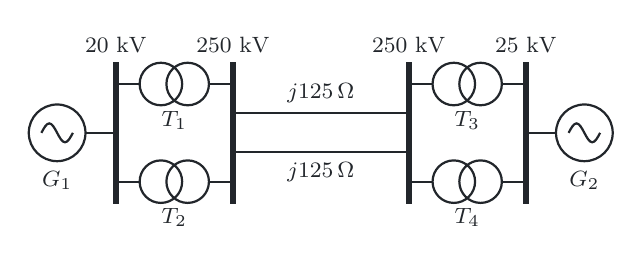
\begin{tikzpicture}[scale=0.62]\circuitoQcinquentaum{0.62}\end{tikzpicture}}

% ---------------------------------------------------------------------
%  Figura: zonas de tensão base da Questão 51 (sobre o mesmo unifilar)
%  As zonas aparecem uma por slide (<2>, <3>, <4>); a fronteira entre duas
%  zonas passa pelo meio do transformador que as separa.
%  \zonaQcinquentaum{slide}{x ini}{x fim}{cor}{nome}{V_b em kV}{elementos}
% ---------------------------------------------------------------------
\newcommand{\zonaQcinquentaum}[7]{%
  \only<#1->{%
    \fill[#4!13] (#2,-0.05) rectangle (#3,4.05);
    \node[anchor=south,font=\footnotesize,text=#4!75!black,inner sep=2pt]
      at ({(#2+#3)/2},4.05) {\textbf{#5}: $V_b = #6$~kV};
    \node[anchor=north,align=center,font=\scriptsize,text=Ink,inner sep=2pt]
      at ({(#2+#3)/2},-0.05) {#7};}}
% tracejado interrompido sob cada trafo, onde fica o rótulo T (usa o \dT
% definido por \circuitoQcinquentaum, então vem depois dele na figura)
\newcommand{\fronteiraQcinquentaum}[2]{% {slide}{x do transformador}
  \only<#1->{\draw[Ink!75,line width=0.7pt,dash pattern=on 3pt off 2pt]
    (#2,4.05) -- (#2,3-\dT) (#2,2.45-\dT) -- (#2,1-\dT);}}
\newcommand{\zonasQcinquentaum}{%
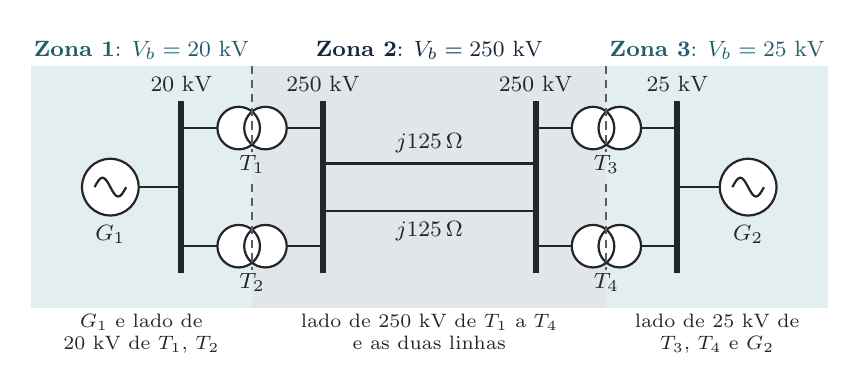
\begin{tikzpicture}[scale=0.75]
  % caixa fixa: a figura não "pula" quando as zonas aparecem
  \path[use as bounding box] (-1.4,-1.0) rectangle (12.2,4.7);
  \zonaQcinquentaum{2}{-1.35}{2.4}{ZonaA}{Zona 1}{20}{$G_1$ e lado de\\20 kV de $T_1$, $T_2$}
  \zonaQcinquentaum{3}{2.4}{8.4}{ZonaB}{Zona 2}{250}{lado de 250 kV de $T_1$ a $T_4$\\e as duas linhas}
  \zonaQcinquentaum{4}{8.4}{12.15}{ZonaA}{Zona 3}{25}{lado de 25 kV de\\$T_3$, $T_4$ e $G_2$}
  \circuitoQcinquentaum{0.75}
  \fronteiraQcinquentaum{3}{2.4}
  \fronteiraQcinquentaum{4}{8.4}
\end{tikzpicture}}

% ---------------------------------------------------------------------
%  Figura: circuito equivalente em pu da Questão 51
%  #1 = 0 -> sistema completo ; #1 = 1 -> linha 2 fora de operação
% ---------------------------------------------------------------------
\newcommand{\equivQcinquentaum}[1]{%
\begin{circuitikz}[scale=0.74, transform shape, line width=0.7pt]
  % fontes e reatâncias dos geradores
  \draw (0,0) to[sV, l=$E_1\angle\delta$] (0,2.4)
        to[L, l=$j0{,}1$] (2,2.4);
  \draw (10,0) to[sV, l_=$E_2\angle 0^\circ$] (10,2.4)
        to[L, l_=$j0{,}1$] (8,2.4);
  % nós (barras) como ligações verticais
  \foreach \x in {2,4,6,8} \draw (\x,1.7) -- (\x,3.1);
  % T1 // T2
  \draw (2,3.1) to[L, l=$j0{,}2$] (4,3.1);
  \draw (2,1.7) to[L, l_=$j0{,}2$] (4,1.7);
  % LT1 // LT2
  \draw (4,3.1) to[L, l=$j0{,}2$] (6,3.1);
  \ifnum#1=0
    \draw (4,1.7) to[L, l_=$j0{,}2$] (6,1.7);
  \else
    \draw[Mute!50, dashed] (4,1.7) -- (6,1.7);
    \draw[Ember, line width=1.4pt] (4.75,1.45) -- (5.25,1.95) (4.75,1.95) -- (5.25,1.45);
    \node[font=\footnotesize, Ember] at (5,1.05) {aberta};
  \fi
  % T3 // T4
  \draw (6,3.1) to[L, l=$j0{,}2$] (8,3.1);
  \draw (6,1.7) to[L, l_=$j0{,}2$] (8,1.7);
  % referência
  \draw (0,0) -- (10,0);
  % rótulos dos blocos
  \foreach \x/\t in {1/G_1, 3/T_1\parallel T_2, 5/L_1\parallel L_2, 7/T_3\parallel T_4, 9/G_2}
    \node[font=\footnotesize, Teal] at (\x,4.05) {$\t$};
  % rótulos das barras
  \foreach \x/\t in {2/20 kV, 4/250 kV, 6/250 kV, 8/25 kV}
    \node[font=\scriptsize, Mute, fill=Paper, inner sep=1pt] at (\x,0.55) {\t};
\end{circuitikz}}

% ---------------------------------------------------------------------
%  Figura: unifilar da Questão 24
%  [#1] = escala (padrão 0.85)
%  #2 = 0 -> enunciado ; #2 = 1 -> com tensões e fluxos da solução
% ---------------------------------------------------------------------
\newcommand{\unifilarQvintequatro}[2][0.85]{%
\begin{tikzpicture}[scale=#1]
  \draw[fio] (0.36,1) -- (1.2,1);   \pic at (0,1) {gerador};
  \draw[fio] (7.6,1) -- (8.44,1);   \pic at (8.8,1) {gerador};
  \foreach \x in {1.2,4.4,7.6} \draw[barra] (\x,0.35) -- (\x,1.65);
  \foreach \x/\n in {1.2/1,4.4/2,7.6/3} \node[numbarra] at (\x,2.0) {\n};
  \draw[fio] (1.2,1) -- node[rot,above] {$j0{,}2$} (4.4,1);
  \draw[fio] (4.4,1) -- node[rot,above] {$j0{,}2$} (7.6,1);
  % carga
  \draw[fio,-{Latex[length=2.2mm]}] (4.4,0.6) -- (4.85,0.6) -- (4.85,-0.15);
  \node[rot,anchor=north west] at (7.7,0.4) {$S_{G3}=0{,}5$};
  \ifnum#2=1
    % fluxos
    \draw[Ember,line width=1pt,-{Latex[length=2mm]}] (2.0,0.62) -- (3.6,0.62);
    \node[font=\scriptsize,Ember,below] at (2.8,0.6) {$S_{12}=0{,}5$};
    \draw[Ember,line width=1pt,-{Latex[length=2mm]}] (6.8,0.62) -- (5.3,0.62);
    \node[font=\scriptsize,Ember,below] at (6.1,0.6) {$S_{32}=0{,}5$};
    \node[font=\scriptsize,Ember,anchor=north] at (4.85,-0.2) {$S_{c}=1{,}0-j0{,}1$};
    % tensões
    \node[font=\scriptsize,Teal,anchor=south] at (1.2,2.25) {$1\angle 0^\circ$};
    \node[font=\scriptsize,Teal,anchor=south] at (4.4,2.25) {$1{,}005\angle{-5{,}71^\circ}$};
    \node[font=\scriptsize,Teal,anchor=south] at (7.6,2.25) {$1\angle 0^\circ$};
  \fi
\end{tikzpicture}}

% ---------------------------------------------------------------------
%  Revisão do conteúdo: caixa de conceito e figuras
% ---------------------------------------------------------------------
% caixa de fórmula/conceito-chave
\newtcolorbox{conceito}[1][]{colback=Teal!6,colframe=Teal,boxrule=0.6pt,
  arc=2pt,left=6pt,right=6pt,top=3pt,bottom=3pt,#1}
% duas fontes ligadas por uma reatância (equação potência-ângulo)
\newcommand{\duasfontes}{%
\begin{circuitikz}[scale=0.8, transform shape, line width=0.7pt]
  \draw (0,0) to[sV, l=$E_1\angle\delta$] (0,1.8)
        to[L, l=$jX$] (3.6,1.8)
        to[sV, l=$E_2\angle 0^\circ$] (3.6,0) -- (0,0);
  \draw[Ember,line width=1pt,-{Latex[length=2mm]}] (1.2,1.2) -- (2.4,1.2)
    node[midway,below,font=\small] {$P$};
\end{circuitikz}}
% curva potência-ângulo P = Pmax sen(delta); x em graus
\newcommand{\curvaPdelta}{%
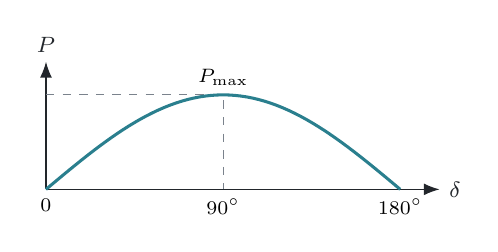
\begin{tikzpicture}[x=0.025cm, y=1.2cm, >={Latex[length=2mm]}]
  \draw[->,Ink] (0,0) -- (200,0) node[right,font=\footnotesize] {$\delta$};
  \draw[->,Ink] (0,0) -- (0,1.35) node[above,font=\footnotesize] {$P$};
  \draw[Mute,dashed] (0,1) -- (90,1) -- (90,0);
  \draw[Teal,line width=1.1pt,domain=0:180,samples=61] plot (\x,{sin(\x)});
  \node[above,font=\scriptsize] at (90,1) {$P_{\max}$};
  \node[below,font=\scriptsize] at (0,0) {$0$};
  \node[below,font=\scriptsize] at (90,0) {$90^\circ$};
  \node[below,font=\scriptsize] at (180,0) {$180^\circ$};
\end{tikzpicture}}
% linha k-m só com reatância (fluxo numa linha)
\newcommand{\linhaKM}{%
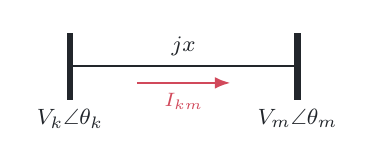
\begin{tikzpicture}[scale=0.85]
  \draw[barra] (0,0.3) -- (0,1.3);
  \draw[barra] (3.4,0.3) -- (3.4,1.3);
  \draw[fio] (0,0.8) -- node[rot,above] {$jx$} (3.4,0.8);
  \draw[Ember,line width=0.9pt,-{Latex[length=2mm]}] (1.0,0.55) -- (2.4,0.55)
    node[midway,below,font=\scriptsize] {$I_{km}$};
  \node[rot,below] at (0,0.3) {$V_k\angle\theta_k$};
  \node[rot,below] at (3.4,0.3) {$V_m\angle\theta_m$};
\end{tikzpicture}}

% ---------------------------------------------------------------------
%  Questão 45: curva de potência instantânea (pgfplots)
%  p(t) = 500 - 1000 cos(2wt - 60°), w = 100*pi rad/s (f = 50 Hz);
%  em graus, 2wt = 36000 t.
%  \graficoQquarentacinco[opções do axis]{0 = enunciado | 1 = com P e S}
% ---------------------------------------------------------------------
\pgfplotsset{
  q45/.style={
    width=7cm, height=5.5cm,
    xmin=0, xmax=0.02, ymin=-600, ymax=1600,
    xtick={0,0.002,0.004,0.006,0.008,0.01,0.012,0.014,0.016,0.018,0.02},
    ytick={-600,-400,...,1600},
    scaled x ticks=false,
    grid=major, major grid style={densely dotted,Ink!40},
    xlabel={tempo em segundos}, ylabel={watt},
    tick label style={font=\tiny,Ink}, label style={font=\scriptsize,Ink},
    xticklabel style={/pgf/number format/.cd,fixed,precision=3,use comma,/tikz/.cd},
    yticklabel style={/pgf/number format/.cd,use comma,1000 sep={}},
    axis line style={Ink}, tick style={Ink!70},
  },
  % rótulos do tempo inclinados (slides, onde a figura é estreita)
  q45 girado/.style={xticklabel style={rotate=45,anchor=north east,inner sep=1pt}},
}
\newcommand{\graficoQquarentacinco}[2][]{%
\begin{tikzpicture}
\begin{axis}[q45,#1]
  \addplot[Ink,line width=1pt,domain=0:0.02,samples=241]
    {500 - 1000*cos(36000*x - 60)};
  \ifnum#2=1
    \draw[Mute,line width=0.5pt] (axis cs:0,1500) -- (axis cs:0.02,1500)
                                 (axis cs:0,-500) -- (axis cs:0.02,-500);
    \addplot[CorP,line width=1pt,dashed,domain=0:0.02] {500};
    \draw[CorS,line width=1pt,{Latex[length=1.8mm]}-{Latex[length=1.8mm]}]
      (axis cs:0.00667,500) -- (axis cs:0.00667,1500)
      node[midway,right,font=\scriptsize] {$S$};
    \draw[CorS,line width=1pt,{Latex[length=1.8mm]}-{Latex[length=1.8mm]}]
      (axis cs:0.01167,500) -- (axis cs:0.01167,-500)
      node[midway,left,font=\scriptsize] {$S$};
    \node[CorP,font=\scriptsize,fill=white,inner sep=1pt,anchor=west]
      at (axis cs:0.0128,500) {$P$};
    \node[font=\scriptsize,Ink,anchor=north west,inner sep=1.5pt]
      at (axis cs:0.0085,1500) {$p_{\max}\approx 1500$};
    \node[font=\scriptsize,Ink,anchor=south east,inner sep=1pt]
      at (axis cs:0.0198,-500) {$p_{\min}\approx -500$};
  \fi
\end{axis}
\end{tikzpicture}}
% triângulo de potências
\newcommand{\trianguloPotencias}{%
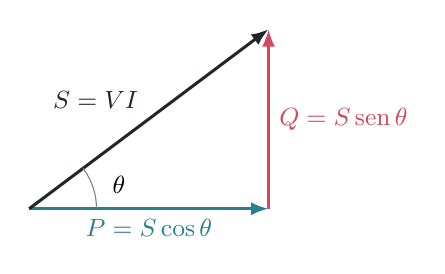
\begin{tikzpicture}[scale=0.95, >={Latex[length=2.2mm]}]
  \draw[->,CorP,line width=1.1pt] (0,0) -- (3.2,0)
    node[midway,below,font=\small] {$P = S\cos\theta$};
  \draw[->,CorS,line width=1.1pt] (3.2,0) -- (3.2,2.4)
    node[midway,right,font=\small] {$Q = S\sen\theta$};
  \draw[->,Ink,line width=1.1pt] (0,0) -- (3.2,2.4)
    node[midway,above left,font=\small] {$S = VI$};
  \draw[Mute] (0.9,0) arc (0:36.87:0.9);
  \node[font=\small] at (1.2,0.32) {$\theta$};
\end{tikzpicture}}

% ---------------------------------------------------------------------
\title{Resolução de Exercícios}
\subtitle{Sistemas Elétricos de Potência --- Questões 51, 24 e 45}
\author{Luis Felipe Souza}
\date{}

\begin{document}

\maketitle

% =====================================================================
\section{Questão 51 --- Perda de uma linha de transmissão}
% =====================================================================

\begin{frame}{Questão 51 --- Enunciado}
  \begin{columns}[c]
    \begin{column}{0.54\textwidth}
      \centering\unifilarQcinquentaum
    \end{column}
    \begin{column}{0.44\textwidth}
      \footnotesize
      Dados dos componentes:\\[0.2em]
      Gerador $G_1$: 100 MVA, 20 kV, $X = 10\%$\\
      Gerador $G_2$: 100 MVA, 25 kV, $X = 10\%$\\
      Transformadores $T_1$ e $T_2$:\\
      \quad 50 MVA, 20 kV/250 kV, $X = 10\%$\\
      Transformadores $T_3$ e $T_4$:\\
      \quad 50 MVA, 25 kV/250 kV, $X = 10\%$
    \end{column}
  \end{columns}

  \vspace{0.8em}
  \small
  A figura acima apresenta um sistema de potência sem perdas. Suponha que,
  inicialmente, a potência ativa transmitida do gerador $G_1$ para o $G_2$
  seja igual a 1,0~p.u., e que os dois estejam operando em suas tensões
  nominais. Em um dado instante, uma das linhas de transmissão é perdida.
  Supondo que as tensões dos geradores e a abertura angular permaneçam
  inalteradas, qual será a nova potência ativa transmitida, em p.u., nessa
  condição de regime?
\end{frame}

\begin{frame}{Questão 51 --- Conteúdos envolvidos}
  Essa questão envolve conceitos de \alert{estabilidade de SEP} e
  \alert{sistema por unidade}:
  \begin{itemize}
    \item \passo{Sistema por unidade (pu)} os dados estão em \% na base de
          cada equipamento, em três níveis de tensão (20, 250 e 25~kV); é
          preciso levá-los a uma base comum.
    \item \passo{Associação de reatâncias} transformadores e linhas em
          paralelo, em série com os geradores, formam a reatância
          equivalente $X_{eq}$.
    \item \passo{Potência transmitida entre duas fontes} a equação
          potência-ângulo, da estabilidade de SEP, mostra como a potência
          depende das tensões, da abertura angular e de $X_{eq}$.
  \end{itemize}
\end{frame}

\begin{frame}{Questão 51 --- Revisão: sistema por unidade}
  \small
  \begin{columns}[T]
    \begin{column}{0.42\textwidth}
      \passo{Definição}
      \[
        \text{valor em pu} = \frac{\text{valor real}}{\text{valor base}}
      \]
      Em \%: $X = 10\,\% \Rightarrow 0{,}10$~pu na base do equipamento.

      \vspace{0.6em}
      \passo{Bases} escolhem-se $S_b$ (trifásica, uma só para todo o
      sistema) e $V_b$ (de linha, uma por zona); as outras saem delas:
      \[
        Z_b = \frac{V_b^2}{S_b}, \qquad I_b = \frac{S_b}{\sqrt{3}\,V_b}
      \]
    \end{column}
    \begin{column}{0.55\textwidth}
      \pause
      \passo{Zonas} ao atravessar um transformador, $V_b$ muda na relação de
      transformação (ex.: 20~kV $\to$ 250~kV); $S_b$ não muda.

      \vspace{0.6em}\pause
      \passo{Mudança de base} os dados de placa vêm na base do próprio
      equipamento:
      \begin{conceito}[left=3pt,right=3pt]
        \centering
        $Z_{\text{pu,novo}} = Z_{\text{pu,velho}}
        \left(\dfrac{S_{b,\text{novo}}}{S_{b,\text{velho}}}\right)
        \left(\dfrac{V_{b,\text{velho}}}{V_{b,\text{novo}}}\right)^{2}$
      \end{conceito}
      \pause
      \passo{Vantagem} com as $V_b$ na relação do transformador, ele fica
      1:1 em pu: no circuito sobra só a sua reatância.
    \end{column}
  \end{columns}
  \vfill
  {\footnotesize\color{Mute} Ver \cite{stevenson1986elementos,bichels2018sep}.}
\end{frame}

\begin{frame}{Questão 51 --- Revisão: equação potência-ângulo}
  \small
  \begin{columns}[T]
    \begin{column}{0.47\textwidth}
      \centering
      \duasfontes
      \[
        I = \frac{E_1\angle\delta - E_2\angle 0^\circ}{jX}
        \;\Rightarrow\;
        P = \operatorname{Re}\{E_1\angle\delta\; I^{*}\}
      \]
      \begin{conceito}
        \centering $P = \dfrac{E_1\,E_2}{X}\,\sin\delta$
      \end{conceito}
    \end{column}
    \begin{column}{0.49\textwidth}
      \pause
      \centering
      \curvaPdelta

      \raggedright
      \begin{itemize}
        \item $\delta$: abertura angular; $X$: reatância total entre as
              fontes;
        \item sem perdas: a potência que sai de uma fonte chega inteira à
              outra;
        \item $P_{\max} = E_1E_2/X$ em $\delta = 90^\circ$: limite de
              estabilidade em regime permanente.
      \end{itemize}
    \end{column}
  \end{columns}
  \vfill
  {\footnotesize\color{Mute} Ver \cite{stevenson1986elementos}.}
\end{frame}

\begin{frame}{Questão 51 --- Estratégia}
  Num sistema sem perdas, a potência transferida entre duas fontes é
  \[
    P = \frac{E_1\,E_2}{X_{eq}}\,\sin\delta .
  \]
  \pause
  Se $E_1$, $E_2$ e $\delta$ \alert{não mudam}, então $P\propto 1/X_{eq}$:
  \[
    \boxed{\;P' = P\,\frac{X_{eq}}{X_{eq}'}\;}
  \]
  \pause
  Basta, portanto:
  \begin{enumerate}
    \item escolher as bases e passar tudo para pu;
    \item calcular $X_{eq}$ antes e depois da perda da linha.
  \end{enumerate}
\end{frame}

\begin{frame}{Questão 51 --- Passo 1: zonas do circuito}
  \small
  \passo{Ideia} Os transformadores dividem o sistema em \alert{zonas}: dentro
  de uma zona a tensão base é uma só; ao atravessar um transformador, ela
  muda na relação de transformação.

  {\centering\zonasQcinquentaum\par}

  \onslide<5->{A fronteira passa \emph{por dentro} de cada transformador: cada
  enrolamento fica na zona da sua tensão nominal (20 kV $\to$ zona 1,
  250 kV $\to$ zona 2, 25 kV $\to$ zona 3).}
\end{frame}

\begin{frame}{Questão 51 --- Passo 1: bases}
  \begin{columns}[c]
    \begin{column}{0.48\textwidth}
      \passo{Potência base} $S_b = 100$~MVA (comum a todo o sistema)

      \vspace{0.6em}\pause
      \passo{Tensões base} definidas pelas relações dos transformadores:
      \begin{itemize}
        \item zona de $G_1$: 20 kV
        \item zona das linhas: 250 kV
        \item zona de $G_2$: 25 kV
      \end{itemize}
    \end{column}
    \begin{column}{0.48\textwidth}
      \pause
      \passo{Impedância base} na zona das linhas:
      \[
        Z_b = \frac{V_b^2}{S_b} = \frac{(250)^2}{100} = 625~\Omega
      \]
      \pause
      \small As tensões nominais dos equipamentos coincidem com as tensões
      base de suas zonas, então só a potência base precisa ser corrigida.
    \end{column}
  \end{columns}
\end{frame}

\begin{frame}{Questão 51 --- Passo 2: reatâncias em pu}
  Mudança de base:\quad
  $X_{\text{novo}} = X_{\text{velho}}
   \left(\dfrac{S_{b,\text{novo}}}{S_{b,\text{velho}}}\right)
   \left(\dfrac{V_{b,\text{velho}}}{V_{b,\text{novo}}}\right)^{2}$

  \vspace{0.8em}
  \begin{tabular}{@{}lll@{}}
    \toprule
    Elemento & Cálculo & $X$ (pu) \\ \midrule
    \pause
    $G_1$, $G_2$ & já estão em 100 MVA e tensão nominal & $0{,}10$ \\
    \pause
    $T_1 \dots T_4$ & $0{,}10 \times \dfrac{100}{50}$ & $0{,}20$ \\[0.6em]
    \pause
    Cada linha & $\dfrac{125}{625}$ & $0{,}20$ \\
    \bottomrule
  \end{tabular}
\end{frame}

\begin{frame}{Questão 51 --- Passo 3: circuito equivalente antes da falha}
  \centering
  \equivQcinquentaum{0}

  \vspace{0.3em}\pause
  \raggedright
  Cada par em paralelo vale $0{,}2\parallel 0{,}2 = 0{,}1$:
  \[
    X_{eq} = \underbrace{0{,}1}_{G_1} + \underbrace{0{,}1}_{T_1\parallel T_2}
           + \underbrace{0{,}1}_{L_1\parallel L_2} + \underbrace{0{,}1}_{T_3\parallel T_4}
           + \underbrace{0{,}1}_{G_2} = \alert{0{,}5~\text{pu}}
  \]
\end{frame}

\begin{frame}{Questão 51 --- Passo 4: circuito equivalente após a perda da linha}
  \centering
  \equivQcinquentaum{1}

  \vspace{0.3em}\pause
  \raggedright
  Só o bloco das linhas muda: agora resta uma linha de $0{,}2$~pu.
  \[
    X_{eq}' = 0{,}1 + 0{,}1 + \alert{0{,}2} + 0{,}1 + 0{,}1 = \alert{0{,}6~\text{pu}}
  \]
\end{frame}

\begin{frame}{Questão 51 --- Resultado}
  \vspace*{-0.4em}
  \[
    P' = P\,\frac{X_{eq}}{X_{eq}'} = 1{,}0 \times \frac{0{,}5}{0{,}6}
  \]
  \begin{resposta}
    \centering $P' = \dfrac{5}{6} \approx 0{,}833$~pu
  \end{resposta}
  \pause
  \passo{Conferência} Com $E_1=E_2=1{,}0$: $\sin\delta = P\,X_{eq} = 0{,}5
  \Rightarrow \delta = 30^\circ$. Depois: $P' = \sin 30^\circ / 0{,}6 = 0{,}833$~pu.

  \vspace{0.3em}\pause
  \passo{Por que não cai pela metade?} A linha perdida é só uma parte da
  reatância total: $X_{eq}$ sobe de $0{,}5$ para $0{,}6$ (20\,\%), e a potência
  cai na mesma proporção inversa.

  \vspace{0.3em}\pause
  {\footnotesize\color{Mute} Obs.: se as tensões mantidas fossem as \emph{terminais}
  dos geradores (sem $X_G$ no caminho), seria $0{,}3/0{,}4 = 0{,}75$~pu.}
\end{frame}

% =====================================================================
\section{Questão 24 --- Fluxo de potência em três barras}
% =====================================================================

\begin{frame}{Questão 24 --- Enunciado}
  \small
  Considere um sistema elétrico de potência representado pelo diagrama
  unifilar a seguir. A potência injetada na barra 3 e as impedâncias das
  linhas que conectam a barra 1 à barra 2 bem como a barra 2 à barra 3 são
  mensuradas por unidade (pu). Tanto a tensão na barra 1 quanto a tensão na
  barra 3 são iguais a 1,0~pu.

  \vspace{0.3em}
  \begin{columns}[c]
    \begin{column}{0.53\textwidth}
      \centering
      {\footnotesize\bfseries Diagrama unifilar do sistema}\\[0.3em]
      \unifilarQvintequatro[0.70]{0}
    \end{column}
    \begin{column}{0.45\textwidth}
      Com base nessas informações, é correto dizer que a tensão na barra 2
      e o fluxo de potência saindo da barra 1 para a barra 2 são,
      respectivamente,
      \begin{enumerate}[(A)]\setlength{\itemsep}{0pt}
        \item $1{,}0$ pu e $1{,}0$ pu.
        \item $1{,}0-j0{,}1$ pu e $1{,}0$ pu.
        \item $1{,}0+j0{,}1$ pu e $0{,}5$ pu.
        \item $1{,}0-j0{,}1$ pu e $0{,}5$ pu.
        \item $1{,}0+j0{,}1$ pu e $1{,}0$ pu.
      \end{enumerate}
    \end{column}
  \end{columns}
\end{frame}

\begin{frame}{Questão 24 --- Conteúdos envolvidos}
  Essa questão envolve conceitos de \alert{fluxo de potência}:
  \begin{itemize}
    \item \passo{Sistema por unidade} tensões, impedâncias e potência já vêm
          em pu (revisto na Questão 51): as contas são feitas direto com eles.
    \item \passo{Fasores e potência complexa} relação entre a potência, a
          tensão e a corrente numa barra.
    \item \passo{Fluxo numa linha} queda de tensão na reatância da linha e
          potência que sai de uma barra para a outra.
  \end{itemize}
\end{frame}

\begin{frame}{Questão 24 --- Revisão: potência complexa e fluxo numa linha}
  \small
  \begin{columns}[T]
    \begin{column}{0.47\textwidth}
      \passo{Potência complexa} injetada na barra $k$:
      \[
        S_k = P_k + jQ_k = V_k\,I_k^{*}
        \;\Rightarrow\;
        I_k = \left(\frac{S_k}{V_k}\right)^{\!*}
      \]

      \pause
      \passo{Linha $k$--$m$} só com reatância $x$:

      {\centering\linhaKM\\[0.4em]
       $V_k - V_m = jx\,I_{km}, \qquad S_{km} = V_k\,I_{km}^{*}$\par}
    \end{column}
    \begin{column}{0.49\textwidth}
      \pause
      \passo{Em módulo e ângulo} com $\theta_{km} = \theta_k - \theta_m$:
      \begin{conceito}
        $P_{km} = \dfrac{|V_k|\,|V_m|}{x}\,\sin\theta_{km}$\\[0.3em]
        $Q_{km} = \dfrac{|V_k|^2 - |V_k|\,|V_m|\cos\theta_{km}}{x}$
      \end{conceito}
      \pause
      \begin{itemize}
        \item $P$ vai do \alert{maior ângulo} para o menor;
        \item a linha consome reativo: $Q_{km} + Q_{mk} = |I_{km}|^2\,x$;
        \item é a equação potência-ângulo da Questão 51.
      \end{itemize}
    \end{column}
  \end{columns}
  \vfill
  {\footnotesize\color{Mute} Ver \cite{stevenson1986elementos,bichels2018sep,borges2005analise}.}
\end{frame}

\begin{frame}{Questão 24 --- Leitura dos dados}
  \begin{itemize}
    \item $V_1 = V_3 = 1{,}0\angle 0^\circ$ pu \quad (fasores dados como $1{,}0$)
    \item $S_{G3} = 0{,}5 + j0$ pu \quad (só potência ativa)
    \item $x = 0{,}2$ pu em cada trecho
  \end{itemize}
  \pause
  \vspace{0.6em}
  \passo{Ideia} A carga da barra 2 é desconhecida, mas na \alert{barra 3}
  conhecemos tensão \emph{e} potência. Daí sai a corrente do trecho 3--2,
  depois $V_2$ e, por fim, o fluxo 1--2.
\end{frame}

\begin{frame}{Questão 24 --- Passos 1 e 2: corrente e tensão na barra 2}
  \passo{Passo 1} Corrente que sai da barra 3 em direção à barra 2:
  \[
    I_{32} = \left(\frac{S_{G3}}{V_3}\right)^{\!*}
           = \left(\frac{0{,}5}{1\angle 0^\circ}\right)^{\!*} = 0{,}5\angle 0^\circ~\text{pu}
  \]
  \pause
  \passo{Passo 2} Queda no trecho 3--2:
  \[
    V_2 = V_3 - jx\,I_{32} = 1 - j0{,}2 \times 0{,}5
        = \alert{1{,}0 - j0{,}1~\text{pu}}
  \]
  \pause
  {\small\color{Mute} Em módulo e ângulo: $|V_2| = 1{,}005$~pu,
  $\theta_2 = -5{,}71^\circ$.}
\end{frame}

\begin{frame}{Questão 24 --- Passo 3: fluxo da barra 1 para a barra 2}
  \[
    I_{12} = \frac{V_1 - V_2}{jx} = \frac{1 - (1 - j0{,}1)}{j0{,}2}
           = \frac{j0{,}1}{j0{,}2} = 0{,}5~\text{pu}
  \]
  \pause
  \[
    S_{12} = V_1\, I_{12}^{*} = 1 \times 0{,}5 = \alert{0{,}5 + j0~\text{pu}}
  \]
  \pause
  \begin{resposta}
    \centering Alternativa \textbf{(D)}:\quad $V_2 = 1{,}0 - j0{,}1$~pu
    \quad e \quad $S_{12} = 0{,}5$~pu
  \end{resposta}
\end{frame}

\begin{frame}{Questão 24 --- Diagrama fasorial (em escala)}
  \centering
  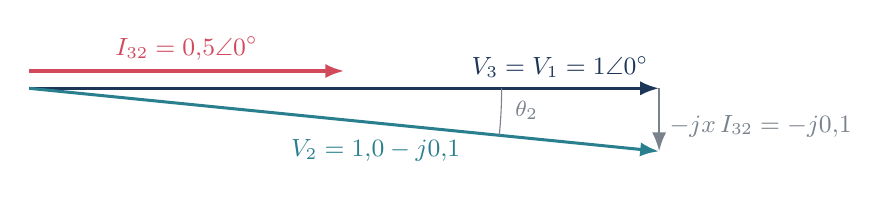
\begin{tikzpicture}[>={Latex[length=2.4mm]}]
    \draw[->,Navy,line width=1.1pt] (0,0) -- (8,0)
      node[above left,font=\small] {$V_3 = V_1 = 1\angle 0^\circ$};
    \draw[->,Ember,line width=1.1pt] (0,0.22) -- node[above,font=\small] {$I_{32} = 0{,}5\angle 0^\circ$} (4,0.22);
    \draw[->,Mute,line width=0.9pt] (8,0) -- (8,-0.8)
      node[right,font=\small,pos=0.6] {$-jx\,I_{32} = -j0{,}1$};
    \draw[->,Teal,line width=1.1pt] (0,0) -- (8,-0.8)
      node[below,font=\small,pos=0.55,yshift=-2pt] {$V_2 = 1{,}0 - j0{,}1$};
    \draw[Mute] (6,0) arc (0:-5.71:6);
    \node[font=\footnotesize,Mute,anchor=west] at (6.05,-0.28) {$\theta_2$};
  \end{tikzpicture}

  \vspace{0.8em}\raggedright\small
  \begin{itemize}
    \pause
    \item $S_{G3}$ é puramente ativa e $|V_3|=1$ $\Rightarrow$ $I_{32}$ fica
          \alert{em fase} com $V_3$.
    \pause
    \item A queda $jx\,I_{32}$ é perpendicular à corrente: altera quase só o
          \emph{ângulo} de $V_2$ ($\theta_2 = -5{,}71^\circ$); o módulo vai a $1{,}005$.
    \pause
    \item Conferência pela fórmula de transferência:
          $P_{12} = \dfrac{|V_1||V_2|}{x}\sin\theta_{12}
          = \dfrac{1 \times 1{,}005}{0{,}2}\,\sin 5{,}71^\circ = 0{,}5$~pu.
  \end{itemize}
\end{frame}

\begin{frame}{Questão 24 --- Interpretação física}
  \centering
  \unifilarQvintequatro{1}

  \vspace{0.6em}\raggedright
  \small
  \begin{itemize}
    \item Simetria: $V_1 = V_3$ e trechos iguais $\Rightarrow$ cada lado entrega
          $0{,}5$ pu à carga ($P_c = 1{,}0$ pu).
    \item Cada trecho consome $Q = |I|^2 x = 0{,}05$; como as fontes não
          entregam reativo, os $0{,}1$ pu vêm da barra 2 (carga capacitiva).
    \pause
    \item (C) e (E) falham: com $V_2 = 1 + j0{,}1$, $I_{12} = -0{,}5$ e o
          fluxo seria de 2 para 1.
  \end{itemize}
\end{frame}

% =====================================================================
\section{Questão 45 --- Potência ativa e reativa}
% =====================================================================

\begin{frame}{Questão 45 --- Enunciado}
  \small
  Sejam $v(t) = \sqrt{2}\,V\sen(\omega t)$ e $i(t) = \sqrt{2}\,I\sen(\omega t
  - \theta)$, respectivamente, a tensão (volts) e a corrente (ampères)
  fornecidas por um gerador CA (Corrente Alternada) em regime permanente.

  A figura apresenta a curva de potência instantânea fornecida por este
  gerador durante o intervalo de tempo $\dfrac{2\pi}{\omega}$.

  {\centering\graficoQquarentacinco[q45 girado,width=8.6cm,height=4.5cm]{0}\par}
\end{frame}

\begin{frame}{Questão 45 --- Enunciado (continuação)}
  \footnotesize
  \begin{columns}[c]
    \begin{column}{0.45\textwidth}
      \centering
      \graficoQquarentacinco[q45 girado,width=6.4cm,height=4.8cm]{0}
    \end{column}
    \begin{column}{0.53\textwidth}
      Denomina-se Potência Ativa $P$ o valor médio da potência instantânea
      ao longo do tempo e é dada por:\\
      $P = VI\cos\theta$.

      Denomina-se Potência Reativa $Q$ o valor calculado pela expressão
      $Q = VI\sen\theta$.

      Analisando a figura, qual o valor aproximado da Potência Reativa, em
      var?
      \begin{enumerate}[(A)]\setlength{\itemsep}{0pt}
        \item 1\,000
        \item 870
        \item 500
        \item 290
        \item Impossível determinar com os dados fornecidos.
      \end{enumerate}
    \end{column}
  \end{columns}
\end{frame}

\begin{frame}{Questão 45 --- Conteúdos envolvidos}
  Essa questão envolve conceitos de \alert{potência em circuitos de corrente
  alternada}:
  \begin{itemize}
    \item \passo{Potência instantânea} o produto $p(t) = v(t)\,i(t)$ de uma
          tensão e uma corrente senoidais, e o que cada parte da curva
          significa.
    \item \passo{Potências ativa, reativa e aparente} $P$, $Q$ e $S = VI$,
          ligadas pelo triângulo de potências.
    \item \passo{Leitura de gráfico} valor médio e amplitude de uma senoide
          deslocada do zero, a partir do máximo e do mínimo.
  \end{itemize}
\end{frame}

\begin{frame}{Questão 45 --- Revisão: potência instantânea}
  \small
  \begin{columns}[T]
    \begin{column}{0.50\textwidth}
      Com $v = \sqrt{2}\,V\sen\omega t$ e $i = \sqrt{2}\,I\sen(\omega t -
      \theta)$:
      \[
        p(t) = v\,i = 2VI\sen(\omega t)\,\sen(\omega t - \theta)
      \]
      Usando $2\sen a\,\sen b = \cos(a-b) - \cos(a+b)$:
      \begin{conceito}[left=3pt,right=3pt]
        \centering
        $p(t) = {\underbrace{VI\cos\theta}_{P}}
              - {\underbrace{VI}_{S}}\cos(2\omega t - \theta)$
      \end{conceito}
    \end{column}
    \begin{column}{0.46\textwidth}
      \pause
      \begin{itemize}
        \item oscila com $2\omega$: o dobro da frequência de $v$ e $i$;
        \item valor médio: $VI\cos\theta = P$;
        \item amplitude: $VI = S$ (potência aparente);
        \item $p_{\max} = P + S$ \ e \ $p_{\min} = P - S$;
        \item $p < 0$: o gerador recebe energia de volta da carga.
      \end{itemize}
    \end{column}
  \end{columns}
  \vfill
  {\footnotesize\color{Mute} Ver \cite{stevenson1986elementos}.}
\end{frame}

\begin{frame}{Questão 45 --- Revisão: potências ativa, reativa e aparente}
  \small
  \begin{columns}[c]
    \begin{column}{0.40\textwidth}
      \centering\trianguloPotencias
    \end{column}
    \begin{column}{0.57\textwidth}
      \begin{itemize}
        \item aparente: $S = VI$ (VA);
        \item ativa: $P = S\cos\theta$ (W), o valor médio de $p(t)$;
        \item reativa: $Q = S\sen\theta$ (var), a amplitude da energia
              que vai e volta entre gerador e carga.
      \end{itemize}
      \begin{conceito}
        \centering $S^2 = P^2 + Q^2$ \quad (pois $\cos^2\theta + \sen^2\theta
        = 1$)
      \end{conceito}
      \pause
      $\theta > 0$: corrente atrasada da tensão $\Rightarrow$ $Q > 0$ (carga
      indutiva). Com fasores ($V\angle 0^\circ$, $I\angle{-\theta}$):
      $V I^{*} = VI\angle\theta = P + jQ$ (Questão 24).
    \end{column}
  \end{columns}
  \vfill
  {\footnotesize\color{Mute} Ver \cite{stevenson1986elementos}.}
\end{frame}

\begin{frame}{Questão 45 --- Passos 1 e 2: $P$ e $S$ pelo gráfico}
  \begin{columns}[c]
    \begin{column}{0.52\textwidth}
      \centering
      \graficoQquarentacinco[q45 girado,width=7.2cm,height=5.6cm]{1}
    \end{column}
    \begin{column}{0.46\textwidth}
      \small
      \passo{Ideia} $p(t) = P - S\cos(2\omega t - \theta)$ é uma senoide
      deslocada: média $P$, amplitude $S$.

      \vspace{0.4em}\pause
      \passo{Leitura} $p_{\max} \approx 1500$~W e $p_{\min} \approx -500$~W.

      \vspace{0.4em}\pause
      \passo{Passo 1}
      $P = \dfrac{p_{\max} + p_{\min}}{2} = \dfrac{1500 - 500}{2}
         = \alert{500~\text{W}}$

      \vspace{0.4em}\pause
      \passo{Passo 2}
      $S = \dfrac{p_{\max} - p_{\min}}{2} = \dfrac{1500 + 500}{2}
         = \alert{1000~\text{VA}}$
    \end{column}
  \end{columns}
\end{frame}

\begin{frame}{Questão 45 --- Passo 3: potência reativa}
  \passo{Ângulo}
  \[
    \cos\theta = \frac{P}{S} = \frac{500}{1000} = 0{,}5
    \quad\Longrightarrow\quad \theta = 60^\circ
  \]
  \pause
  \passo{Reativa}
  \[
    Q = S\sen\theta = 1000 \times \sen 60^\circ = 1000 \times 0{,}866
      \approx 866~\text{var}
  \]
  \pause
  {\small Ou, pelo triângulo: $Q = \sqrt{S^2 - P^2} = \sqrt{1000^2 - 500^2}
  = \sqrt{750\,000} \approx 866$~var.}
  \pause
  \begin{resposta}
    \centering Alternativa \textbf{(B)}:\quad $Q \approx 866~\text{var}
    \approx 870$~var
  \end{resposta}
\end{frame}

\begin{frame}{Questão 45 --- Conferências}
  \small
  \begin{itemize}
    \item \passo{Sinal de $\theta$} $p(0) = 0$ e a curva começa
          \emph{descendo}: $p'(0) = -2\omega VI\sen\theta < 0
          \Rightarrow \sen\theta > 0$. Logo $\theta = +60^\circ$: corrente
          atrasada, $Q > 0$.
    \pause
    \item \passo{Tempos} $2\pi/\omega = 0{,}02$~s $\Rightarrow$ $\omega =
          100\pi$~rad/s (50~Hz). Mínimo em $t = \theta/(2\omega) = 1/600
          \approx 0{,}0017$~s; máximo em $t = (\theta + \pi)/(2\omega) =
          1/150 \approx 0{,}0067$~s: batem com o gráfico.
    \pause
    \item \passo{Distratores} (C) $500$ é $P$; (A) $1000$ é $S$; (D)
          $\approx 289$ sairia de $P\,\mathrm{tg}\,30^\circ$ (ângulo
          errado). Não é (E): o gráfico não dá $V$ e $I$ separados, mas dá o
          produto $VI$, que é o que importa.
  \end{itemize}
\end{frame}

% =====================================================================
\begin{frame}[standout]
  \begin{tabular}{rl}
    Q51 & $P' \approx 0{,}833$ pu \\[0.4em]
    Q24 & Alternativa (D) \\[0.4em]
    Q45 & Alternativa (B)
  \end{tabular}
\end{frame}

% =====================================================================
\begin{frame}[allowframebreaks]{Referências}
  \nocite{bichels2018sep,borges2005analise,stevenson1986elementos}
  \printbibliography[heading=none]
\end{frame}

\end{document}
